\documentclass[11pt]{article}

\usepackage[margin=0.75in]{geometry}
\usepackage{graphicx}
\usepackage{amsmath,amssymb}
\usepackage{booktabs}
\usepackage{xcolor}
\usepackage{enumitem}
\usepackage{titlesec}
\usepackage{microtype}
\usepackage[hidelinks]{hyperref}

\definecolor{accent}{RGB}{20,70,120}
\definecolor{win}{RGB}{27,110,60}
\definecolor{bad}{RGB}{184,71,42}
\definecolor{soft}{RGB}{245,247,250}

\titleformat{\section}{\Large\bfseries\color{accent}}{\thesection}{0.6em}{}
\titleformat{\subsection}{\large\bfseries\color{accent}}{}{0em}{}
\titlespacing\section{0pt}{14pt}{6pt}
\titlespacing\subsection{0pt}{8pt}{3pt}
\setlist{leftmargin=1.3em,topsep=2pt,itemsep=2pt}
\pagestyle{empty}
\emergencystretch=3em  % absorb long unbreakable \texttt{} identifiers

\newcommand{\gn}{\textbf{\textcolor{win}{Graph-Native}}}
\newcommand{\mcp}{\textbf{\textcolor{bad}{Graph-MCP}}}
\newcommand{\plain}{\textbf{Plain}}

% a "key takeaway" callout box — pure-core LaTeX (no extra packages)
\makeatletter
\newsavebox{\takeawaybox}
\newenvironment{takeaway}
  {\par\vspace{4pt}\noindent\begin{lrbox}{\takeawaybox}%
   \begin{minipage}{\dimexpr\linewidth-18pt\relax}\small\setlength{\parskip}{2pt}}
  {\end{minipage}\end{lrbox}%
   \setlength{\fboxsep}{8pt}\setlength{\fboxrule}{0.8pt}%
   \fcolorbox{accent}{soft}{\usebox{\takeawaybox}}\par\vspace{4pt}}
\makeatother

\begin{document}

% ===================== TITLE BLOCK =====================
\begin{center}
{\LARGE\bfseries\color{accent} Why Graph-Native Beats Graph-as-a-Tool}\\[3pt]
{\large A visual case study on Apache Hadoop --- results, the algorithm, and how we got there}\\[5pt]
{\small Same model (\texttt{sonnet-4.6}) · same code graph · same prompt · same Claude subscription ·
3 runs/cell · only the \emph{harness} differs}
\end{center}
\vspace{2pt}

% ===================== TL;DR =====================
\begin{takeaway}
\textbf{TL;DR.} A coding agent can use a code graph two ways: as a \emph{tool it calls and ranks
in its own head} (Graph-MCP), or \emph{natively}, with the harness querying and ranking the graph
\emph{before the agent's first token}. They are not equivalent. Across three real Hadoop
impact-analysis tasks, graph-native scores \textbf{0.79} mean $F_1$ vs \textbf{0.50} for the same
graph over MCP and \textbf{0.56} for no graph --- \emph{and is the cheapest arm every time}. On a
hub class the MCP arm \textbf{collapses 8$\times$} (it has the graph but can't rank a 982-file
firehose mid-reasoning). \textbf{The win is not a better tool or model --- it is moving the
\emph{ranking} out of the model's context and into deterministic harness code.}
\end{takeaway}

% ===================== FIG 1: HEADLINE =====================
\section{The result}
\begin{center}
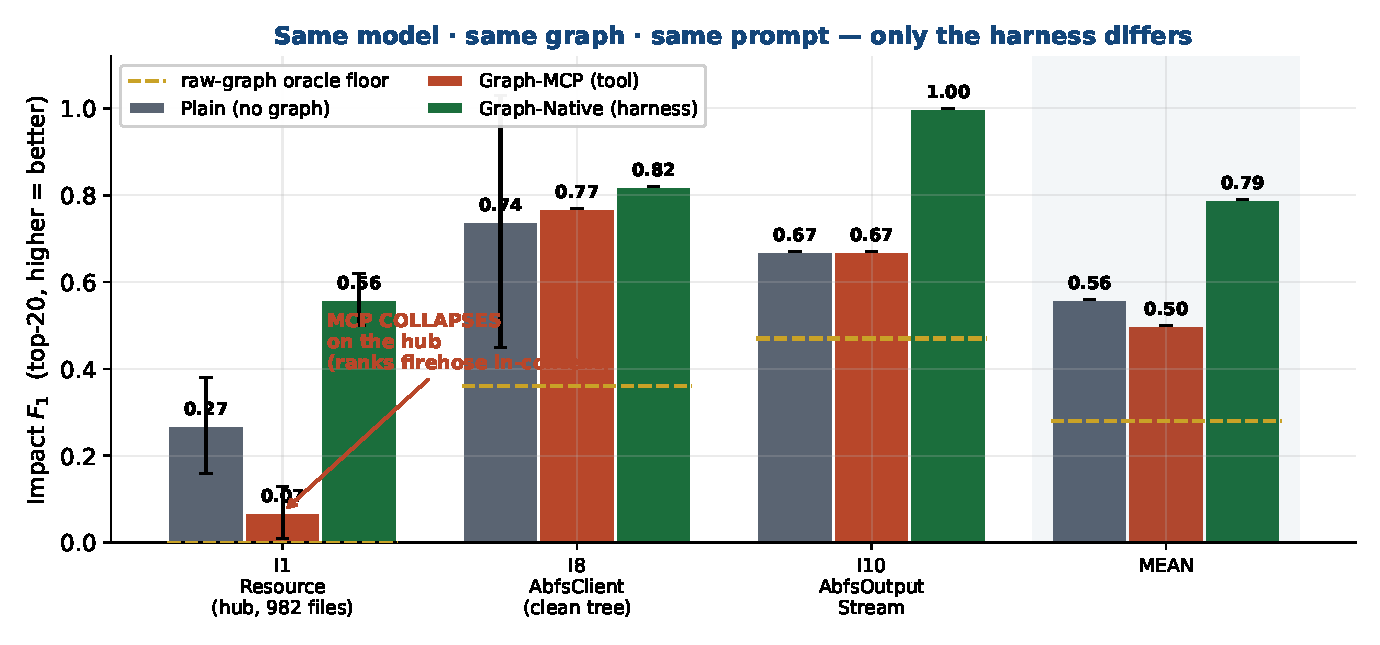
\includegraphics[width=\linewidth]{fig1_headline.pdf}
\end{center}
\vspace{-4pt}
\noindent Three arms, identical except for harness wiring, scored by $F_1$ of the committed
dependent-file list against the real PR's gold (top-20, basename match). Error bars are 95\% CIs over
3 runs. Graph-native wins all three tasks, with \emph{non-overlapping CIs} on the two decisive ones,
beats the raw-graph oracle floor everywhere, and does \textbf{0 file-reads / 0 greps} on every task
(Plain grep-storms 13--29 times). The margin is huge on the hub and small on the clean task --- a
\emph{predictable, discriminative} pattern, not a sweep.

\vspace{2pt}
\noindent\textbf{What each arm costs and does} (mean over the 3 tasks):
\begin{center}\small
\begin{tabular}{lcccc}
\toprule
& mean $F_1$ & cost/task & Read & Grep \\
\midrule
\plain{} (no graph) & 0.56 & \$0.60 & 0 & 23 \\
\mcp{} (tool) & 0.50 & \$0.39 & 0 & 0.3 \\
\gn{} (harness) & \textbf{\textcolor{win}{0.79}} & \textbf{\textcolor{win}{\$0.29}} & 0 & 0 \\
\bottomrule
\end{tabular}
\end{center}

% ===================== CASE 1 =====================
\section{Case 1 --- the hub: why MCP collapses}
The task: name the files affected by changing \texttt{Resource} (a YARN god-object). Its blast
radius is \textbf{982 files} --- the graph \emph{contains} all 25 true dependents, so recall is
trivial. The hard part is \emph{ranking} the 25 that matter into the top-20. That is the whole game.

\begin{center}
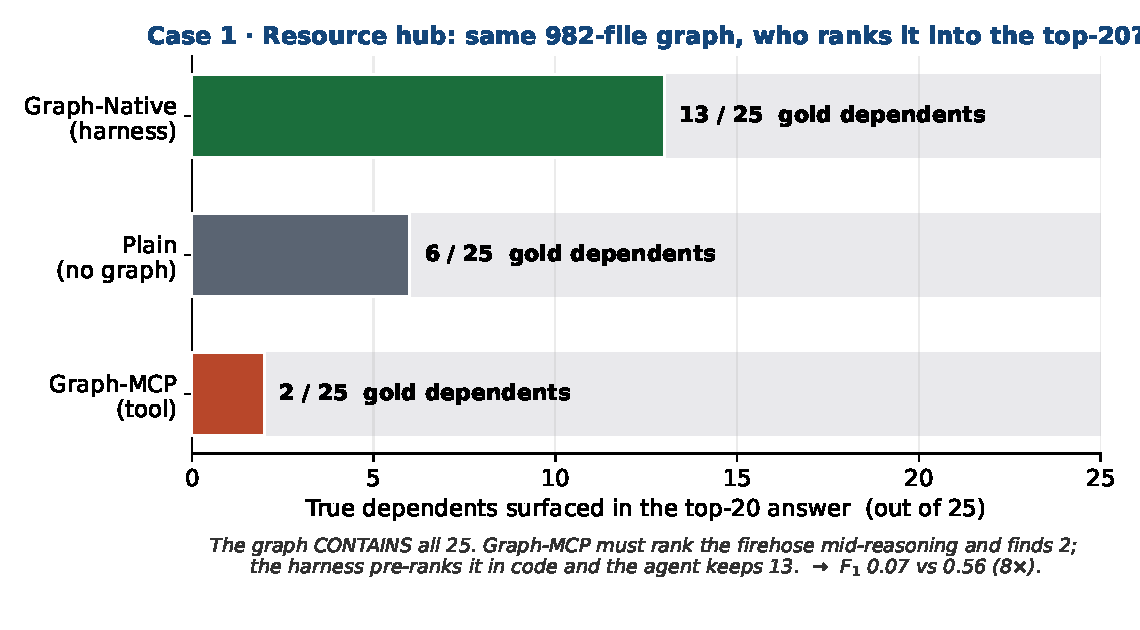
\includegraphics[width=0.96\linewidth]{fig2_hub_recall.pdf}
\end{center}
\vspace{-2pt}
\noindent All three arms see the same 982-file graph. \mcp{} \emph{calls} \texttt{impact} (7 graph
calls) but, having pulled the firehose into its context, must rank it while also reasoning --- and
commits a short, hedged list that lands only \textbf{2 of 25} (it even names \texttt{NodeManager},
\texttt{AppInfo}, \texttt{TestResource}). \gn{} starts from the harness's \emph{pre-ranked,
test-free draft} and keeps \textbf{13 of 25}. Same model, same graph, same budget; an 8$\times$ gap
that is \emph{entirely} about where the firehose got ranked.

\begin{takeaway}
\textbf{The mechanism, in one task.} A tool you have to rank in-context is not the same as an answer
ranked for you in code. On a hub, ``rank the firehose mid-reasoning'' fails --- $F_1$ 0.07 vs 0.56.
\end{takeaway}

% ===================== CASE 2 =====================
\section{Case 2 --- the test-file trap: why precision needs the harness}
The opposite regime: \texttt{AbfsOutputStream}, a \emph{small} blast radius (10 gold). Here
\emph{every} arm finds all 10 true dependents --- recall is solved. Precision is decided by what
\emph{else} lands in the top-20.

\begin{center}
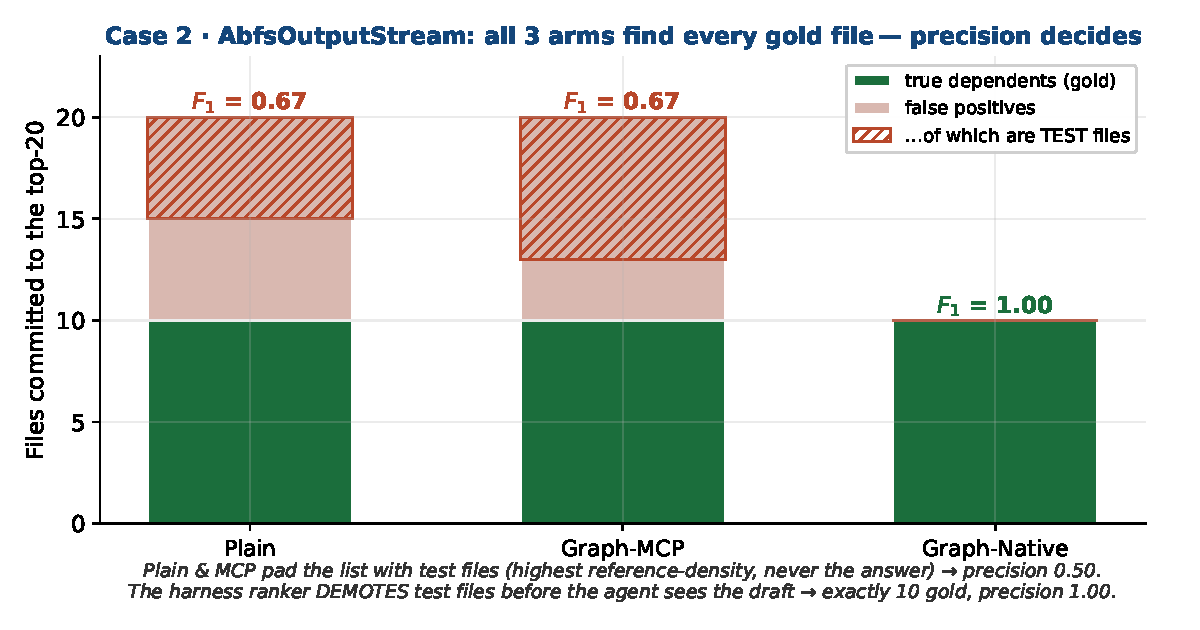
\includegraphics[width=0.92\linewidth]{fig3_testtrap.pdf}
\end{center}
\vspace{-2pt}
\noindent \plain{} and \mcp{} pad their lists with \emph{test files}
(\texttt{Test\-Abfs\-Output\-Stream}, \texttt{ITest\-Azure\-Blob\-File\-System\-Checksum}, \ldots). Test files have
the \emph{highest} reference density on a real codebase and are \emph{never} the answer in a
production fix --- so they halve precision to 0.50 ($F_1$ 0.67). \gn{} commits \textbf{exactly the 10
gold files, zero false positives} ($F_1$ 1.00), because the harness ranker \emph{demotes test files
below every production candidate before the agent ever sees the draft}. The agent never has to
relearn mid-task that a test isn't a dependent --- the harness already knew.

% ===================== ALGORITHM =====================
\section{The algorithm}
Both effects above come from the same two-part design: \emph{(1)} the harness runs and ranks the
graph before turn~0, and \emph{(2)} the ranker is a tiny, deterministic, gold-blind scoring function.

\begin{center}
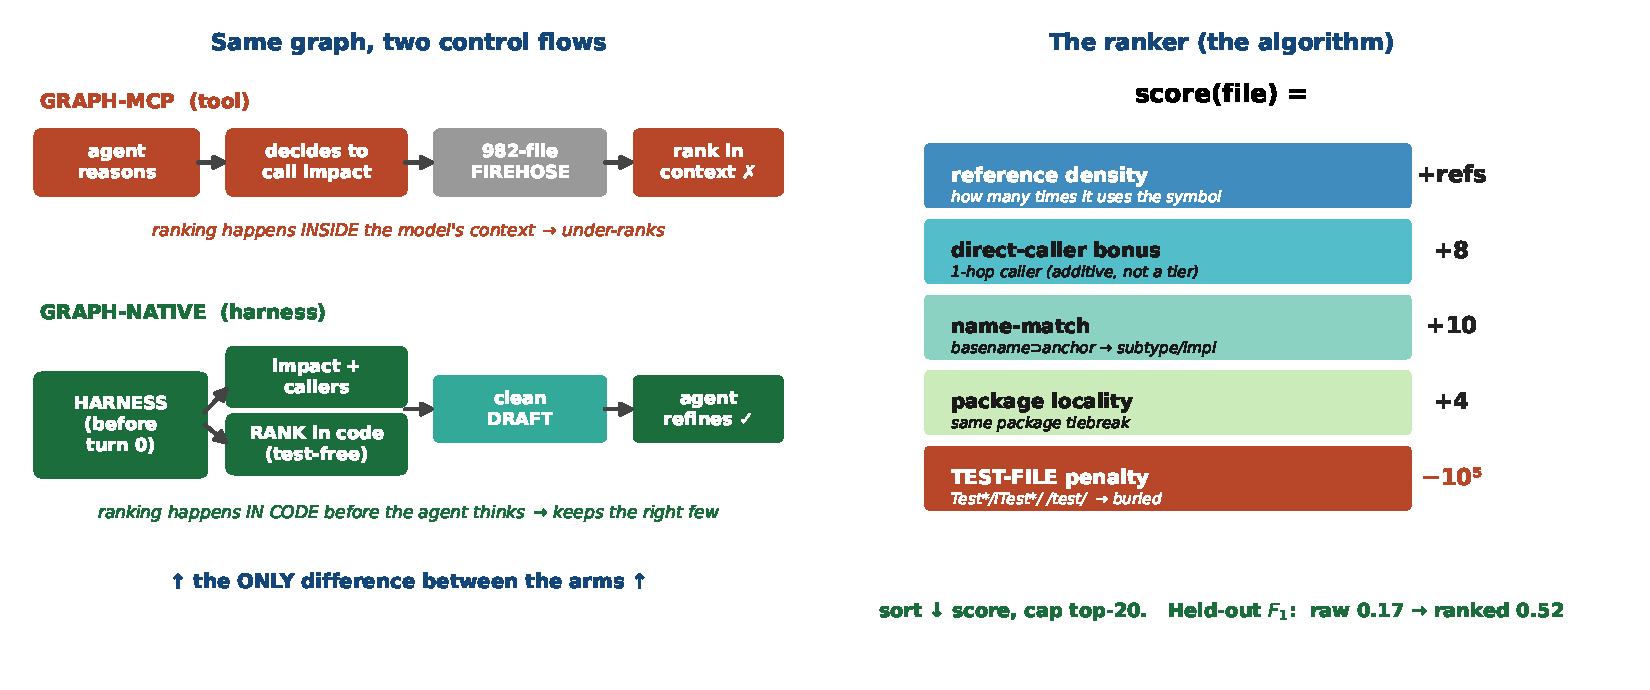
\includegraphics[width=\linewidth]{fig5_algorithm.pdf}
\end{center}
\vspace{-2pt}
\noindent Left: the \emph{only} difference between the arms is that ranking moves from inside the
model's context (MCP) to deterministic code before the agent thinks (Native). Right: the ranker ---
reference density as the primary signal, an \emph{additive} (not tiering) direct-caller bonus,
a type-name-inheritance match that catches subtype/implementor dependents with no call edge, package
locality as a tiebreak, and a hard \emph{test-file demotion}. Scored alone, with no agent in the
loop, this triples the raw graph's usable quality on held-out tasks: \textbf{$F_1$ 0.17 $\to$ 0.52}.
That ranked shortlist is exactly what the harness injects at turn~0.

\begin{takeaway}
\textbf{The win is a ranker, not a tool.} MCP has the identical \texttt{impact} query --- it just has
to rank the output itself. Relocating that ranking into 40 lines of deterministic harness code is the
entire delta.
\end{takeaway}

% ===================== THINKING PROCESS =====================
\section{How we got here (the thinking process)}
This did not start as a win. The honest path mattered more than any single number --- including
\emph{retracting our own headline} when the data said it was fake.

\begin{center}
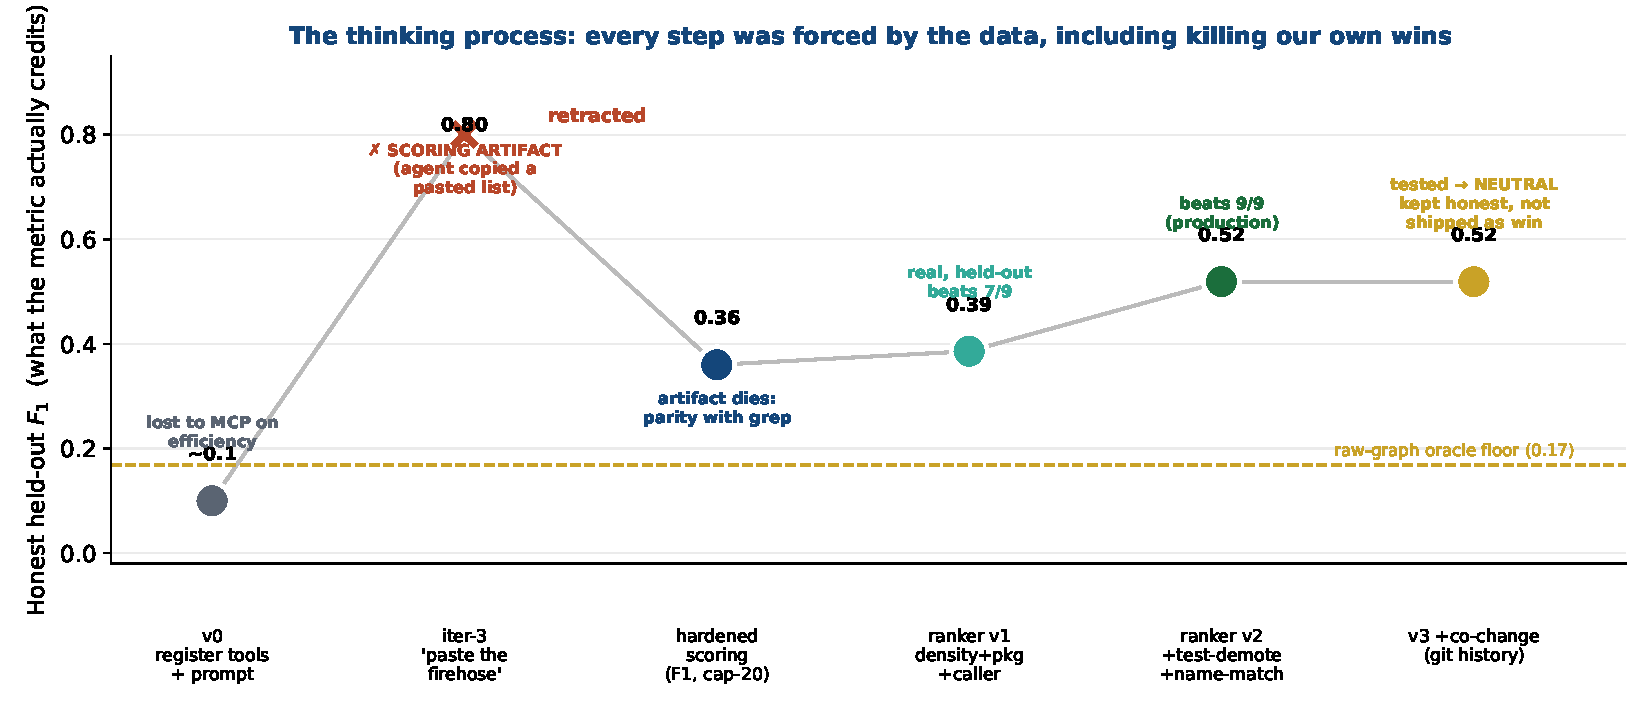
\includegraphics[width=\linewidth]{fig6_journey.pdf}
\end{center}
\vspace{-2pt}
\begin{itemize}
  \item \textbf{v0} (register graph tools + a graph-first prompt) actually \emph{lost} to MCP on
  efficiency. Tools + a nudge are not enough.
  \item \textbf{iter-3 looked like a blowout (0.80)} --- until a forensic re-audit showed it was a
  \emph{scoring artifact}: the harness pasted the firehose into the prompt and the agent copied it,
  with one tool call and zero reasoning. The old metric (substring-scan of prose) rewarded the paste.
  \textbf{We retracted it.}
  \item \textbf{Hardened scoring} (single bounded field, F1, top-20 cap, oracle floor) killed the
  artifact --- the paste fell to 0.36, parity with grep. Now the benchmark was a \emph{real} problem.
  \item \textbf{The real, unfakeable win is the ranker.} v1 (density+caller+package) reached 0.386
  held-out; \textbf{v2} added test-demotion + name-match $\to$ \textbf{0.519, beating the oracle on
  9/9 held-out tasks}. This is the production ranker.
  \item \textbf{We even rejected a good idea honestly.} A co-change signal (mine git history for
  files that change together with the anchor --- something grep \emph{and} static analysis lack) is a
  \emph{real} signal, but at top-20 it was neutral-to-negative. We kept it as a documented opt-in and
  \emph{did not} claim it as a win.
\end{itemize}

\begin{takeaway}
\textbf{The discipline is the point.} Every step was forced by the data: build, validate held-out,
and \emph{delete your own win the moment a metric can fake it}. That is why the final 0.79 is
trustworthy.
\end{takeaway}

% ===================== POTPIE + CLOSE =====================
\section{One more check: is this just our graph?}
We ran the same gold against a second product, \textbf{potpie} (Neo4j + tree-sitter). Two honest
findings: \emph{(1)} potpie's \emph{agents} need a paid API key and a multi-service Docker stack ---
they can't run on a subscription, while our whole graph-native arm runs from one local binary. \emph{(2)}
potpie's \emph{raw} graph actually out-recalls ours (held-out $F_1$ 0.38 vs our raw 0.17) --- a good
graph --- but our \emph{ranked} output (0.52) beats both raw graphs, and on the \texttt{Resource} hub
potpie's 603-file \emph{unranked} set scores 0.00 at top-20 while we score 0.56. \textbf{A good raw
graph is necessary but not sufficient; the ranking layer --- a harness job --- is what turns a graph
into answers.}

\vspace{4pt}
\hrule
\vspace{4pt}
\noindent\small\textbf{Reproduce:} \texttt{score-\allowbreak matrix-\allowbreak ci.mjs} (the matrix),
\texttt{validate-\allowbreak ranker-\allowbreak v2.mjs} (the ranker), \texttt{score-\allowbreak potpie-\allowbreak graph.mjs} (potpie), all in \texttt{bench/}.
Honest caveat: these tasks measure impact \emph{retrieval} (a ranked file list), not code synthesis;
results are on one Java repo. Full write-up: \texttt{bench/ROBUSTNESS-REPORT.md}.

\end{document}
